\documentclass{article}
\usepackage[utf8x]{inputenc}
\usepackage{ucs}
\usepackage{amsmath} 
\usepackage{amsfonts}
\usepackage{upgreek}
\usepackage[english,russian]{babel}
\usepackage{graphicx}
\usepackage{float}
\usepackage{textcomp}
\usepackage{hyperref}
\usepackage{geometry}
  \geometry{left=2cm}
  \geometry{right=1.5cm}
  \geometry{top=1cm}
  \geometry{bottom=2cm}
\usepackage{tikz}
\usepackage{ccaption}
\usepackage{multicol}

\usepackage{listings}
%\setlength{\columnsep}{1.5cm}
%\setlength{\columnseprule}{0.2pt}

\definecolor{solcolor}{RGB}{226,240,245}

\begin{document}
\pagenumbering{gobble}

\lstset{
  language=C,                % choose the language of the code
  basicstyle=\linespread{1.1}\ttfamily,
  columns=fixed,
  fontadjust=true,
  basewidth=0.5em,
  keywordstyle=\color{blue}\bfseries,
  commentstyle=\color{gray},
  stringstyle=\ttfamily\color{orange!50!black},
  showstringspaces=false,
  %numbers=false,                   % where to put the line-numbers
  numbersep=5pt,
  numberstyle=\tiny\color{black},
  numberfirstline=true,
  stepnumber=1,                   % the step between two line-numbers.        
  numbersep=10pt,                  % how far the line-numbers are from the code
  backgroundcolor=\color{white},  % choose the background color. You must add \usepackage{color}
  showstringspaces=false,         % underline spaces within strings
  captionpos=b,                   % sets the caption-position to bottom
  breaklines=true,                % sets automatic line breaking
  breakatwhitespace=true,         % sets if automatic breaks should only happen at whitespace
  xleftmargin=.2in,
  frame=tlbr,
  framesep=14pt,
  framerule=0pt,
  extendedchars=\true,
  keepspaces = true,
}
\lstset{literate=%
   *{0}{{{\color{red!20!violet}0}}}1
    {1}{{{\color{red!20!violet}1}}}1
    {2}{{{\color{red!20!violet}2}}}1
    {3}{{{\color{red!20!violet}3}}}1
    {4}{{{\color{red!20!violet}4}}}1
    {5}{{{\color{red!20!violet}5}}}1
    {6}{{{\color{red!20!violet}6}}}1
    {7}{{{\color{red!20!violet}7}}}1
    {8}{{{\color{red!20!violet}8}}}1
    {9}{{{\color{red!20!violet}9}}}1
}

\title{Семинар \#1: Основы C. Решения классных задач. \vspace{-5ex}}\date{}\maketitle
\section*{Часть 2: Основы C}
\subsection*{Hello World!}
Простейшая программа на языке C выглядит следующим образом:
\begin{lstlisting}
#include <stdio.h>
int main() {
    printf("Hello world!");
}
\end{lstlisting}

Эта программа печатает на экран строку "Hello world!".
\begin{itemize}
\item \texttt{\#include <stdio.h>}  - включаем библиотеку stdio (standard input/output), которая содержит \texttt{printf}.
\item \texttt{int main() \{ ... \}} - основная функция программы, с неё начинается исполнение любой программы.
\item \texttt{printf("Hello world!");} - печатаем на экран.
\end{itemize}

\subsection*{Задание на основы \texttt{printf}}
\begin{enumerate}
\item Скомпилируйте программу, используя \texttt{gcc} и запустите.
\item В строке функции \texttt{printf()} можно использовать некоторые специальные символы \texttt{\textbackslash n}, \texttt{\textbackslash t} и \texttt{\textbackslash b}. Добавьте эти символы в строку функции \texttt{printf} (в произвольное место) и выясните, что они делают.
\item Напишите программу, которая будет выводить на экран:
\begin{verbatim}
First
    Second
        Third
\end{verbatim}
Используйте 1 вызов функции \texttt{printf}. Для отступов используйте пробелы или знаки табуляции(\texttt{\textbackslash t}).

\begin{lstlisting}[backgroundcolor = \color{solcolor}]
#include <stdio.h>
int main() {
    printf("First\n\tSecond\n\t\tThird\n");
}
\end{lstlisting}
\end{enumerate}

\subsection*{Целочисленные переменные \texttt{int}:}
В переменных \texttt{int} можно хранить целые числа от $-2^{31}$ до $2^{31} - 1$. ($2^{31}$ примерно равно двум миллиардам)
\begin{lstlisting}
#include <stdio.h>
int main() {
    int a;
    int b = 5;
    a = 3;
    int res = a * b + (b / a);
    printf("Result = %i\n", res);
}
\end{lstlisting}

\begin{itemize}
\item \texttt{int a} - Объявляем, что у нас есть переменная a, которая будет хранить целые числа.
\item \texttt{int b = 5} - Объявляем, что есть переменная b, которая будет хранить целые числа и присваиваем ей 5.
\item \texttt{a = 3} - Присваиваем переменной a число 3.
\item \texttt{res = a * b + (b / a)} - Сохраняем в переменной res результат вычислений.
\item \texttt{printf(``Result = \%i \textbackslash n '', res)} Печатаем, за место спецификатора \texttt{\%i} (сокращение от \texttt{int}) подставится значение переменной.
\end{itemize}
\subsection*{Задание на целочисленные переменные:}
\begin{enumerate}
\item Создайте переменные \texttt{a} и \texttt{b} и присвойте им значения \texttt{a = 26}, а \texttt{b = 7}. Затем:
\begin{itemize}
\item Напечатайте на экран число \texttt{a}. Вот так:
\begin{lstlisting}[backgroundcolor = \color{solcolor}]
#include <stdio.h>
int main() {
	int a = 26, b = 7;
	printf("%i\n");
}
\end{lstlisting}
\item Напечатайте на экран 2 числа \texttt{a} и \texttt{b}, разделённые пробелом. Вот так:
\begin{lstlisting}[backgroundcolor = \color{solcolor}]
#include <stdio.h>
int main() {
	int a = 26, b = 7;
	printf("%i %i\n", a, b);
}
\end{lstlisting}

\item Напечатайте на экран 2 числа \texttt{a} и \texttt{b} в следующем формате \texttt{(26, 7)}.
\begin{lstlisting}[backgroundcolor = \color{solcolor}]
#include <stdio.h>
int main() {
	int a = 26, b = 7;
	printf("(%i, %i)\n", a, b);
}
\end{lstlisting}

\item Напечатайте на экран 2 числа \texttt{a} и \texttt{b} в следующем формате \texttt{[26:7])}.
\begin{lstlisting}[backgroundcolor = \color{solcolor}]
#include <stdio.h>
int main() {
	int a = 26, b = 7;
	printf("[%i:%i]\n", a, b);
}
\end{lstlisting}
\newpage
\item Напечатайте на экран 2 числа \texttt{a} и \texttt{b} в следующем формате \texttt{(A = 26 and B = 7)}.
\begin{lstlisting}[backgroundcolor = \color{solcolor}]
#include <stdio.h>
int main() {
	int a = 26, b = 7;
	printf("A = %i and B = %i\n", a, b);
}
\end{lstlisting}
\item Напечатайте на экран сумму чисел \texttt{a} и \texttt{b}.
\begin{lstlisting}[backgroundcolor = \color{solcolor}]
#include <stdio.h>
int main() {
	int a = 26, b = 7;
	printf("%i\n", a + b);
}
\end{lstlisting}
\item Напечатайте на экран произведение чисел \texttt{a} и \texttt{b}.
\begin{lstlisting}[backgroundcolor = \color{solcolor}]
#include <stdio.h>
int main() {
	int a = 26, b = 7;
	printf("%i\n", a * b);
}
\end{lstlisting}
\item Напечатайте на экран результат целочисленного деления \texttt{a} на \texttt{b}. Используйте оператор: \texttt{a / b}. В результате этой
		операции должно получиться целое число \texttt{3} (так как это операция деления нацело).
\begin{lstlisting}[backgroundcolor = \color{solcolor}]
#include <stdio.h>
int main() {
	int a = 26, b = 7;
	printf("%i\n", a / b);
}
\end{lstlisting}
\item Напечатайте на экран остаток деления \texttt{a} на \texttt{b}. Используйте оператор: \texttt{a \% b}. В результате этой
		операции должно получиться целое число \texttt{5}.
\begin{lstlisting}[backgroundcolor = \color{solcolor}]
#include <stdio.h>
int main() {
	int a = 26, b = 7;
	printf("%i\n", a % b);
}
\end{lstlisting}
	\end{itemize}

\newpage
\item Пусть \texttt{a = 2147483647} (максимальное возможное значение для \texttt{int}). Напечатайте значение \texttt{a + 1} и \texttt{2a}.
\begin{lstlisting}[backgroundcolor = \color{solcolor}]
#include <stdio.h>
int main() {
	int a = 2147483647;
	printf("%i\n%i\n", a + 1, 2 * a);
}
\end{lstlisting}
\end{enumerate}

\section*{Адрес и размер переменной:}
\begin{itemize}
\item 1 бит - минимальная единица измерения памяти. В 1 бите может хранится либо \texttt{0} либо \texttt{1}.
\item Вся память делится на ячейки, размером в 8 бит = 1 байт.
\item Все эти ячейки занумерованы, номер ячейки называется адресом.
\item Все переменные содержатся в памяти. Адрес переменной - это адрес первого байта переменной.
\item Чтобы найти адрес переменной, нужно перед ней поставить \texttt{\&}, например, \texttt{\&a}
\item Чтобы найти размер переменной в байтах: \texttt{sizeof(a)}
\item Например, переменная типа \texttt{int} имеет размер 4 байта = 32 бита. Значит в ней может хранится максимум $2^{32}$ значений.
\end{itemize}

\begin{center}
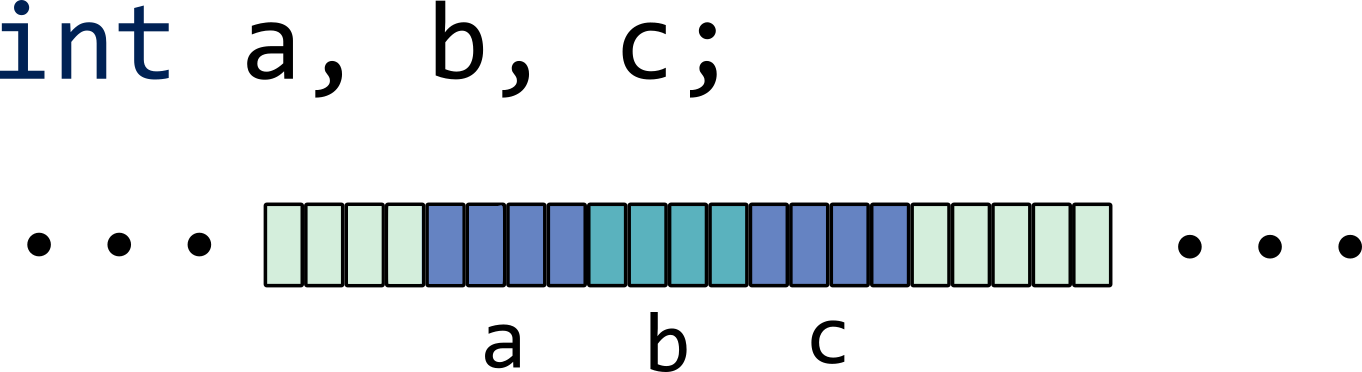
\includegraphics[scale=0.8]{../images/memory_ints.png}
\end{center}

\subsection*{Задание:}
\begin{enumerate}
\item Напечатать размер переменной типа \texttt{int} в байтах. Для этого используйте оператор \texttt{sizeof}:
\begin{lstlisting}[backgroundcolor = \color{solcolor}]
#include <stdio.h>
int main() {
	int a = 26;
	printf("%i\n", sizeof(a));
}
\end{lstlisting}
\item Напечатать адреса переменных типа \texttt{int}. Для этого используйте оператор \texttt{\&}. Адреса памяти обычно хранятся не в переменных типа \texttt{int}, а в больших по размеру переменных. Поэтому для их печати нужно использовать не \texttt{\%i}, а \texttt{\%lli} или \texttt{\%p}.:
\begin{lstlisting}[backgroundcolor = \color{solcolor}]
#include <stdio.h>
int main() {
	int a = 26, b = 7;
	printf("%lli %lli\n", &a, &b);
}
\end{lstlisting}
Убедитесь, что переменные \texttt{a} и \texttt{b} лежат в памяти вплотную друг к другу.
\end{enumerate}

\newpage
\section*{Считывание переменных - scanf:}
Считывание переменных из терминала осуществляется с помощью функции \texttt{scanf} из библиотеки \texttt{stdio}. В отличии от \texttt{printf}, в \texttt{scanf} нужно передавать не саму переменную, а её адрес. Это естественно, так как \texttt{scanf} должен записать считываемое значение в соответствующие ячейки памяти.\\
Пример программы, которая считывает переменные a и b и печатает на экран их произведение:
\begin{lstlisting}
#include <stdio.h>
int main() {
    int a, b;
    scanf("%i", &a); // <-- не забудьте тут амперсанд &
    scanf("%i", &b); // <-- не забудьте тут амперсанд &
    printf("Result = %i\n", a * b);
}
\end{lstlisting}
\textit{Примечание:} При задании формата в \texttt{scanf} не нужно ставить пробелы и символы переноса строки. Т.е. не нужно писать так:
\begin{lstlisting}
scanf("%i\n", &a);  // будет ожидать ввода ещё одного числа
\end{lstlisting}
\subsection*{Задание на считывание:}
\begin{enumerate}
\item Написать программу, которая считывает целое число и печатает на экран квадрат этого числа.
\begin{lstlisting}[backgroundcolor = \color{solcolor}]
#include <stdio.h>
int main() {
	int a;
	scanf("%i", &a);
	printf("%i\n", a * a);
}
\end{lstlisting}
\item Считать 2 целых числа и напечатать результат целочисленного деления первого на второе.

\begin{lstlisting}[backgroundcolor = \color{solcolor}]
#include <stdio.h>
int main() {
	int a, b;
	scanf("%i%i", &a, &b);
	printf("%i\n", a / b);
}
\end{lstlisting}
\item Считать 2 целых числа и напечатать остаток деления первого на второе.
\begin{lstlisting}[backgroundcolor = \color{solcolor}]
#include <stdio.h>
int main() {
	int a, b;
	scanf("%i%i", &a, &b);
	printf("%i\n", a % b);
}
\end{lstlisting}
\item Считать целое число и напечатать его последнюю цифру. Используйте оператор остатка.
\begin{lstlisting}[backgroundcolor = \color{solcolor}]
#include <stdio.h>
int main() {
	int a;
	scanf("%i", &a);
	printf("%i\n", a % 10);
}
\end{lstlisting}
\item На вход подаётся прошедшее время в формате \texttt{hh:mm}, например, \texttt{05:14}. Нужно напечатать, общее количество минут (\texttt{314}). Создайте 2 переменные \texttt{hours} и \texttt{minutes} и считать значения этих переменных с помощью \texttt{scanf}. Вот так:
\begin{lstlisting}[backgroundcolor = \color{solcolor}]
#include <stdio.h>
int main() {
	int hours, minutes;
	scanf("%i:%i", &hours, &minutes);
	printf("%i\n", 60 * hours + minutes);
}
\end{lstlisting}
\end{enumerate}

\section*{Операторы инкремента:}
Для удобства в языке C введены следующие операторы:
\begin{verbatim}
+=    -=    *=    /=     ++   --    и другие
\end{verbatim}
Например оператор присваивания сложения \texttt{+=} увеличивает левый аргумент на величину правого.\\
Оператор \texttt{++} увеличивает значение аргумента на 1.
\begin{lstlisting}
#include <stdio.h>
int main() {
    int a = 100;
    a = a + 5;  // увеличиваем a на 5
    a += 5;     // увеличиваем a на 5 ( то же самое )
    
    a++;        // увеличиваем a на 1
    ++a;        // увеличиваем a на 1
}
\end{lstlisting}
Чему будет равно значение переменной a после выполнение данного кода?


\newpage
\section*{Логические операторы:}
\begin{center}
\texttt{\begin{multicols}{2}
\begin{tabular}{ c c }
 == & равно\\ 
 != & не равно \\  
 > & больше \\  
 >= & больше и равно \\ 
 < & меньше \\
 <= & меньше и равно \\
\end{tabular}
\begin{tabular}{ c c }
 \&\& & логическое И \\ 
 || & логическое ИЛИ \\  
 !  & логическое НЕ \\  
\end{tabular}
\end{multicols}
}
\end{center}

Пример программы, которая считывает возраст человека и печатает \texttt{Yes}, если возраст больше или равен 18:
\begin{lstlisting}
#include <stdio.h>
int main() {
    int age;
    scanf("%i", &age);
    if (age >= 18) {
    	printf("Yes\n");
    }
}
\end{lstlisting}
\quad\\
Пример программы, которая считывает число \texttt{n} и печатает \texttt{Yes}, если число двузначно и \texttt{No} иначе:
\begin{lstlisting}
#include <stdio.h>
int main() {
    int n;
    scanf("%i", &n);
    if (n >= 10 && n < 100) {
       	printf("Yes\n");
    }
    else {
    	printf("No\n");
    }
}
\end{lstlisting}

Пример программы, которая принимает на вход число и печатает \texttt{Positive}, если число положительное, \texttt{Negative}, если число отрицательное и \texttt{Zero}, если число равно нулю:
\begin{lstlisting}
#include <stdio.h>
int main() {
    int n;
    scanf("%i", &n);
    if (n > 0) {
       	printf("Positive\n");
    }
    else if (n == 0){
    	printf("Zero\n");
    }
    else {
    	printf("Negative\n");
    }
}
\end{lstlisting}


\subsection*{Задание на логические операторы:}
\begin{enumerate}
\item Написать программу, которая считывает число и печатает \texttt{Yes}, если число равно \texttt{42} и \texttt{No} иначе. Обратите внимание, что для сравнения чисел нужно использовать оператор \texttt{==} ("два равна").
\begin{lstlisting}[backgroundcolor = \color{solcolor}]
#include <stdio.h>
int main() {
	int a;
	scanf("%i", &a);
	if (a == 42)
		printf("Yes\n");
	else
		printf("No\n");
}
\end{lstlisting}
\item Написать программу, которая принимает на вход число и печатает \texttt{Yes}, если число принадлежит множеству $(-\infty, -12] \cup (97, +\infty)$  и \texttt{No} иначе.
\begin{lstlisting}[backgroundcolor = \color{solcolor}]
#include <stdio.h>
int main() {
	int a;
	scanf("%i", &a);
	if (a <= -12 || a > 97)
		printf("Yes\n");
	else
		printf("No\n");
}
\end{lstlisting}
\item Написать программу, которая принимает на вход число и печатает \texttt{Even}, если число четное и \texttt{Odd}, если число нечетное. Подсказка: число чётное, если остаток от делениея на 2 равен 0.
\begin{lstlisting}[backgroundcolor = \color{solcolor}]
#include <stdio.h>
int main() {
	int a;
	scanf("%i", &a);
	if (a % 2)
		printf("Odd\n");
	else
		printf("Even\n");
}
\end{lstlisting}

\newpage
\item Написать программу, которая принимает на вход два числа и печатает \texttt{First}, если первое число больше второго, \texttt{Second}, если второе больше первого и \texttt{Equal}, если числа равны.
\begin{lstlisting}[backgroundcolor = \color{solcolor}]
#include <stdio.h>
int main() {
	int a, b;
	scanf("%i%i", &a, &b);
	if (a > b)
		printf("First\n");
	else if (a < b)
		printf("Second\n");
	else
		printf("Equal\n");
}
\end{lstlisting}
\item Написать программу, которая принимает на вход два числа и печатает большее из этих двух чисел.
\begin{lstlisting}[backgroundcolor = \color{solcolor}]
#include <stdio.h>
int main() {
	int a, b;
	scanf("%i%i", &a, &b);
	if (a > b)
		printf("%i\n", a);
	else
		printf("%i\n", b);
}
\end{lstlisting}
\item Написать программу, которая принимает на вход три числа и печатает \texttt{Unique}, если все числа различны и \texttt{Not Unique}, если хотя бы 2 числа равны.
\begin{lstlisting}[backgroundcolor = \color{solcolor}]
#include <stdio.h>
int main() {
	int a, b, c;
	scanf("%i%i%i", &a, &b, &c);
	if (a != b && b != c && c != a)
		printf("Unique\n");
	else
		printf("Not Unique\n");
}
\end{lstlisting}
\end{enumerate}

\newpage
\section*{Цикл \texttt{while}:}
\subsubsection*{Пример:}
Пример программы, которая печатает числа от 0 до 9, разделённые пробелом:
\begin{lstlisting}
#include <stdio.h>
int main() {
    int i = 0;
    while (i < 10) {
        printf("%i ", i);
        i += 1;
    }
}
\end{lstlisting}
\subsubsection*{Задачи:}
Измените программу выше так чтобы:
\begin{enumerate}
\item Программа печатала числа от 0 до 20
\begin{lstlisting}[backgroundcolor = \color{solcolor}]
#include <stdio.h>
int main() {
    int i = 0;
    while (i <= 20) {
        printf("%i ", i);
        i += 1;
    }
}
\end{lstlisting}
\item Программа печатала числа от 5 до 15
\begin{lstlisting}[backgroundcolor = \color{solcolor}]
#include <stdio.h>
int main() {
    int i = 5;
    while (i <= 15) {
        printf("%i ", i);
        i += 1;
    }
}
\end{lstlisting}

\newpage
\item Программа печатала числа от 5 до 15, разделённые не пробелом, а запятой:
\begin{verbatim}
5,6,7,8,9,10,11,12,13,14,15,
\end{verbatim}
\begin{lstlisting}[backgroundcolor = \color{solcolor}]
#include <stdio.h>
int main() {
    int i = 5;
    while (i <= 15) {
        printf("%i,", i);
        i += 1;
    }
}
\end{lstlisting}
\item Программа печатала числа, разделённые символом \texttt{+}
\begin{lstlisting}[backgroundcolor = \color{solcolor}]
#include <stdio.h>
int main() {
    int i = 5;
    while (i <= 15) {
        printf("%i+", i);
        i += 1;
    }
}
\end{lstlisting}
\item Программа печатала числа, разделённые символом переноса строки \texttt{\textbackslash n}. (каждое число в новой строке)
\begin{lstlisting}[backgroundcolor = \color{solcolor}]
#include <stdio.h>
int main() {
    int i = 5;
    while (i <= 15) {
        printf("%i\n", i);
        i += 1;
    }
}
\end{lstlisting}
\item Программа печатала квадраты этих чисел
\begin{lstlisting}[backgroundcolor = \color{solcolor}]
#include <stdio.h>
int main() {
    int i = 5;
    while (i <= 15) {
        printf("%i ", i * i);
        i += 1;
    }
}
\end{lstlisting}
\newpage
\item Программа печатала только чётные числа от 0 до 100
\begin{lstlisting}[backgroundcolor = \color{solcolor}]
#include <stdio.h>
int main() {
    int i = 0;
    while (i <= 100) {
        printf("%i ", i);
        i += 2;
    }
}
\end{lstlisting}
\item Программа печатала только числа, делящиеся на 7  (от 0 до 100)
\begin{lstlisting}[backgroundcolor = \color{solcolor}]
#include <stdio.h>
int main() {
    int i = 0;
    while (i <= 100) {
        printf("%i ", i);
        i += 7;
    }
}
\end{lstlisting}
\item Программа должна считывать число \texttt{n} и печатать все числа от \texttt{0} до \texttt{n} через пробел.
\begin{lstlisting}[backgroundcolor = \color{solcolor}]
#include <stdio.h>
int main() {
    int n;
    scanf("%i", &n);
    int i = 0;
    while (i <= n) {
        printf("%i ", i);
        i += 1;
    }
}
\end{lstlisting}
\item Программа должна считывать число \texttt{n} и печатать все квадраты чисел от \texttt{0} до \texttt{n} через перенос строки.
\begin{lstlisting}[backgroundcolor = \color{solcolor}]
#include <stdio.h>
int main() {
    int n;
    scanf("%i", &n);
    int i = 0;
    while (i <= n) {
        printf("%i\n", i * i);
        i += 1;
    }
}
\end{lstlisting}
\item Программа должна считывать число \texttt{n} и для каждого числа из диапазона от \texttt{0} до \texttt{n} программа должна печатать \texttt{Foo}, если число делится на \texttt{3} и \texttt{Bar}, если число делится на \texttt{5}.
\begin{lstlisting}[backgroundcolor = \color{solcolor}]
#include <stdio.h>
int main() {
    int n;
    scanf("%i", &n);
    int i = 0;
    while (i <= n) {
        printf("%i: ", i);
        if (i % 3 == 0)
            printf("Foo");
        if (i % 5 == 0)
            printf("Bar");
        printf("\n");
        i += 1;
    }
}
\end{lstlisting}
\item Программа должна считывать числа \texttt{a}, \texttt{b}, \texttt{c}, и печатать все числа, делящиеся на \texttt{c} на отрезке от \texttt{a} до \texttt{b} через пробел.
\begin{lstlisting}[backgroundcolor = \color{solcolor}]
#include <stdio.h>
int main() {
    int a, b, c;
    scanf("%i%i%i", &a, &b, &c);
    int i = a - 1 + c - (a - 1) % c;
    while (i <= b) {
        printf("%i ", i);
        i += c;
    }
}

\end{lstlisting}
\end{enumerate}

\subsubsection*{Пример:}
Пример программы, которая вычисляет сумму чисел от \texttt{1} до \texttt{n}.
\begin{lstlisting}
#include <stdio.h>
int main() {
    int n;
    scanf("%d", &n);
    int sum = 0;
    int i = 1;
    while (i <= n) {
        sum += i;
        i += 1;
    }
    printf("%d\n", sum);
}
\end{lstlisting}
\subsubsection*{Задачи:}
Измените программу выше так чтобы:
\begin{enumerate}
\item Программа находила произведение всех чисел от \texttt{1} до \texttt{n}.
\begin{lstlisting}[backgroundcolor = \color{solcolor}]
#include <stdio.h>
int main() {
    int n;
    scanf("%d", &n);
    int fact = 1;
    int i = 1;
    while (i <= n) {
        fact *= i;
        i += 1;
    }
    printf("%d\n", fact);
}
\end{lstlisting}
\item Программа находила сумму всех нечётных чисел от \texttt{1} до \texttt{n}.
\begin{lstlisting}[backgroundcolor = \color{solcolor}]
#include <stdio.h>
int main() {
    int n;
    scanf("%d", &n);
    int sum = 0;
    int i = 1;
    while (i <= n) {
        sum += i;
        i += 2;
    }
    printf("%d\n", sum);
}
\end{lstlisting}

\item Программа находила сумму квадратов всех чисел от \texttt{1} до \texttt{n}.
\begin{lstlisting}[backgroundcolor = \color{solcolor}]
#include <stdio.h>
int main() {
    int n;
    scanf("%d", &n);
    int sum = 0;
    int i = 1;
    while (i <= n) {
        sum += i * i;
        i += 1;
    }
    printf("%d\n", sum);
}
\end{lstlisting}
\item Программа вычисляла следующее выражение:
$$
1^2 - 2^2 + 3^2 - 4^2 + 5^2 - 6^2 + ... + (-1)^{n + 1} n^2
$$
\begin{lstlisting}[backgroundcolor = \color{solcolor}]
#include <stdio.h>
int main() {
    int n;
    scanf("%d", &n);
    int sum = 0;
    int i = 1;
    while (i <= n) {
    	if (i % 2)
        	sum += i * i;
        else 
        	sum -= i * i;
        i += 1;
    }
    printf("%d\n", sum);
}
\end{lstlisting}
\end{enumerate}

\subsubsection*{Пример:}
Пример программы, которая считывает числа последовательно и печатает квадраты этих чисел. Если попадётся отрицательное число, то программа закончится.
\begin{lstlisting}
#include <stdio.h>
int main() {
    while (1) {
    	int a;
    	scanf("%i", &a);
    	if (a < 0) {
    		break;
    	}
        printf("%i\n", a * a);
    }
}
\end{lstlisting}

\subsubsection*{Задачи:}
Измените программу выше так чтобы:
\begin{enumerate}
\item Программа выводила кубы чисел, пока не встретит отрицательное число.
\begin{lstlisting}[backgroundcolor = \color{solcolor}]
#include <stdio.h>
int main() {
    while (1) {
    	int a;
    	scanf("%i", &a);
    	if (a < 0) {
    		break;
    	}
        printf("%i\n", a * a * a);
    }
}
\end{lstlisting}
\item Программа печатала \texttt{Odd}, если число нечётное и \texttt{Even}, если число чётное, пока не встретит отрицательное число
\begin{lstlisting}[backgroundcolor = \color{solcolor}]
#include <stdio.h>
int main() {
    while (1) {
    	int a;
    	scanf("%i", &a);
    	if (a < 0) {
    		break;
    	}
    	if (a % 2)
        	printf("Odd\n");
        else
        	printf("Even\n");
    }
}
\end{lstlisting}
\item Для каждого введённого числа \texttt{a} программа должна печатать последовательность чисел от \texttt{1} до \texttt{a} через пробел. Для этого вам нужно использовать ещё один цикл \texttt{while} внутри цикла \texttt{while}.
\begin{lstlisting}[backgroundcolor = \color{solcolor}]
#include <stdio.h>
int main() {
    while (1) {
    	int a;
    	scanf("%i", &a);
    	if (a < 0) {
    		break;
    	}
    	int i = 1;
    	while (i <= a) {
    		printf("%i ", i);
    		i++;
    	}
    	printf("\n");
    }
}
\end{lstlisting}
\newpage
\item Для каждого введённого числа \texttt{a} программа должна печатать сумму последовательности чисел от \texttt{1} до \texttt{a}.
\begin{lstlisting}[backgroundcolor = \color{solcolor}]
#include <stdio.h>
int main() {
    while (1) {
    	int a;
    	scanf("%i", &a);
    	if (a < 0) {
    		break;
    	}
    	int sum = 0;
    	int i = 1;
    	while (i <= a) {
    		sum += i;
    		i++;
    	}
    	printf("%i\n", sum);
    }
}
\end{lstlisting}
\end{enumerate}


\section*{Цикл \texttt{for}:}
\subsubsection*{Пример:}
Пример программы с циклом \texttt{for}, которая печатает числа от \texttt{0} до \texttt{9}.
\begin{lstlisting}
#include <stdio.h>
int main() {
    for (int i = 0; i < 10; ++i) {
        printf("%i ", i);
    }
}
\end{lstlisting}
Для компиляции этой программы возможно потребуется указать опцию компилятора \texttt{-std=c11}. Вот так:
\begin{verbatim}
gcc -o prog -std=c11 <файл исходного кода>
\end{verbatim}

\subsubsection*{Задачи:}
Измените программу выше так чтобы:
\begin{enumerate}
\item Программа печатала числа от 0 до 20
\begin{lstlisting}[backgroundcolor = \color{solcolor}]
#include <stdio.h>
int main() {
    for (int i = 0; i < 21; ++i) {
        printf("%i ", i);
    }
}
\end{lstlisting}

\newpage
\item Программа печатала числа от 5 до 15
\begin{lstlisting}[backgroundcolor = \color{solcolor}]
#include <stdio.h>
int main() {
    for (int i = 5; i <= 15; ++i) {
        printf("%i ", i);
    }
}
\end{lstlisting}
\item Программа печатала числа от 5 до 15, разделённые не пробелом, а запятой:
\begin{verbatim}
5,6,7,8,9,10,11,12,13,14,15,
\end{verbatim}
\begin{lstlisting}[backgroundcolor = \color{solcolor}]
#include <stdio.h>
int main() {
    for (int i = 5; i <= 15; ++i) {
        printf("%i,", i);
    }
}
\end{lstlisting}
\item Программа печатала числа, разделённые символом переноса строки \texttt{\textbackslash n}. (каждое число в новой строке)
\begin{lstlisting}[backgroundcolor = \color{solcolor}]
#include <stdio.h>
int main() {
    for (int i = 5; i <= 15; ++i) {
        printf("%i\n", i);
    }
}
\end{lstlisting}
\item Программа печатала только числа, делящиеся на \texttt{7}  (от \texttt{0} до \texttt{100})
\begin{lstlisting}[backgroundcolor = \color{solcolor}]
#include <stdio.h>
int main() {
    for (int i = 0; i <= 100; i += 7) {
        printf("%i ", i);
    }
}
\end{lstlisting}
\item Программа считывала \texttt{n} и печатала все числа от \texttt{1} до \texttt{n} и их квадраты в следующем виде:
\begin{verbatim}
1 1
2 4
3 9
4 16
...
\end{verbatim}
\begin{lstlisting}[backgroundcolor = \color{solcolor}]
#include <stdio.h>
int main() {
    int n;
    scanf("%i", &n);
    for (int i = 1; i <= n; i += 1) {
        printf("%i %i\n", i, i * i);
    }
}
\end{lstlisting}
\item Программа считывала \texttt{n} и печатала \texttt{n} символов звёздочка \texttt{*}. Например, если ввести \texttt{7}, то программа должна напечатать \texttt{*******}.
\begin{lstlisting}[backgroundcolor = \color{solcolor}]
#include <stdio.h>
int main() {
    int n;
    scanf("%i", &n);
    for (int i = 0; i < n; i++) {
        printf("*");
    }
    printf("\n");
}
\end{lstlisting}
\end{enumerate}

\subsubsection*{Пример:}
Что напечатает данная программа?
\begin{lstlisting}
#include <stdio.h>
int main() {
    int n;
    scanf("%i", &n);
    for (int i = 0; i < n; ++i) {
        for (int j = 0; j < n; ++j) {
            printf("(%i %i) ", i, j);
        }
        printf("\n");
    }
}
\end{lstlisting}

\newpage
\subsubsection*{Задачи:}
Измените программу выше так чтобы:
\begin{enumerate}
\item Программа печатала таблицу умножения.
\begin{lstlisting}[backgroundcolor = \color{solcolor}]
#include <stdio.h>
int main() {
    for (int i = 1; i < 10; i++) {
    	for (int j = 1; j < 10; j++) {
        	printf("%2i ", i * j);
        }
        printf("\n");
    }
}
\end{lstlisting}
\item Программа считывала \texttt{n} и печатала квадрат из звёздочек размером \texttt{nxn}. \\
\textit{Это одна из домашних задач}
\end{enumerate}

\end{document}